\subsection{Die Supply Chain und die Wertschöpfungskette}\label{wsk}
Damit der Weg von Entwicklung, über Bereitstellung und letztendlichen Kauf nachvollzogen werden kann, werden die Schlüsselpartner in Abbildung \hyperref[img:supplychain]{7} in einer Supply Chain dargestellt. Der Prozess startet bei Software Providern, welche eine Idee für eine Software haben und diese umsetzen. Hierzu ist möglicherweise die Zusammenarbeit mit Service Providern notwendig. Die entwickelte Software wird an den Software Shop weitergeleitet und dieser stellt sie entweder im Shop bereit oder nicht. Abschließend können Fahrzeughalter Software über eine kabellose Schnittstelle wie das Telefonnetz der Mobilfunkbetreiber Softwares herunterladen. Die Wertschöpfungskette ist als detailliertere Sicht des "\textit{Software Shops}" (siehe Abb.) zu sehen. Sie stellt die Entscheidungen und Schritte dar, die eine Software von der Lieferung des Providers \textbf{(IN)} bis zum Download im Shop \textbf{OUT} durchlaufen und bestehen muss.
\begin{figure}[!h]
	\centering
	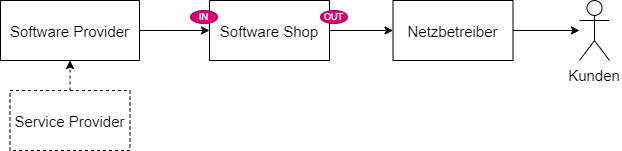
\includegraphics[width=0.9\columnwidth]{pictures/konzept-supplychain.png}
	\label{img:supplychain}
	\caption{Supply Chain von Software}
\end{figure}\\
Nach Porter ist die Wertschöpfungskette in primäre und unterstützende Aktivitäten aufzuteilen.\cite{wsk}Primäre Aktivitäten "liefern dabei einen direkten wertschöpfenden Beitrag zur Erstellung eines Produktes."\cite[Vgl.]{wsk} Unterstützende Aktivitäten sind als "notwendige Voraussetzung zu Erstellung der Produkte"\cite[Vgl. ebd.]{wsk}zu sehen. Sie sind im Rahmen aller Primäraktivitäten aktiv und beeinflussen die Qualität des Produktes. \cite{wsk2}. In Abbildung \hyperref[img:wsk]{8} werden die identifizierten Bausteine den Aktivitäten einer Wertschöpfungskette zugeordnet. Die in Kapitel \ref{key_activities} festgelegte Gruppierung der Schlüsselaktivitäten wird beibehalten und farblich hervorgehoben.

\subsubsection{Primäre Aktivitäten}
Es gibt fünf primäre Aktivitäten. Die erste Aktivität ist die Beschaffung und Lagerung von Materialien, in diesem Fall von Softwares, welche als \textbf{Eingangslogistik} bezeichnet wird. Im Kontext dieser sind zwei wichtige Bausteine zu erwähnen:
\begin{itemize}
	\item[] \hspace{-0.6cm}\textbf{Software-Sicherheit verifizieren}\\ \label{security}
	Sämtliche Softwares die dem Shop hinzugefügt werden sollen, müssen zunächst diverse Sicherheitschecks überstehen. Zum einen sollten Softwares hinsichtlich aufgenommener und gespeicherter Daten überprüft werden. Je nach Land gelten unterschiedliche Datenschutzrichtlinien, welche zu beachten sind um die Privatsphäre von Fahrzeughaltern zu schützen. Weiterhin muss festgestellt werden, dass durch die neue Software keine Sicherheitslücken bei der Fahraufgabe entstehen. Möglicherweise kann dies durch die Nutzung von Simulationen erreicht werden. \\
	Es ist sinnvoll, ein Sicherheitskonzept zu entwickeln welches die Überprüfung von Software unterstützt. Das Ziel des Sicherheitsverifikation ist letzten Endes, dass durch neues Softwares keine Gefahren für die Fahrzeuginsassen entstehen. 
	
	\item[] \hspace{-0.6cm} \textbf{Klassifizierung von Software}\\
	Erfüllt eine Software die Sicherheitsrichtlinen, wird sie anschließend Klassifiziert. Die Klassifizierung von Software soll die Suche und Darstellung dieser im Shop unterstützen, in dem der Software diverse Meta-Daten hinzugefügt werden. Teilweise können diese Meta-Daten im Shop als Such-Filter verwendet werden, einzelne geben auch an wie gut/schlecht eine Software ist und welche Aufgabe sie erfüllt. Ein beispielhaftes Konzept  wird in Kapitel \ref{sw_klassifizierung} erarbeitet und erklärt.
\end{itemize}
\begin{figure}[!h]
	\hspace{-2.5cm}
	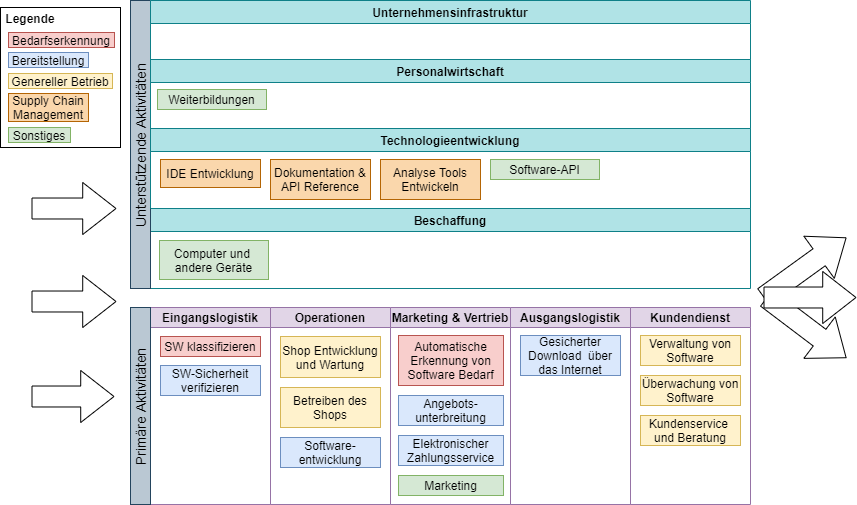
\includegraphics[width=1.2\columnwidth]{pictures/konzept-wsk.png}
	\label{img:wsk}
	\caption{Die wichtigsten Bausteine einzelner Aktivitäten der Wertschöpfungskette}
\end{figure}
Nach erfolgreichen Durchlaufen der Eingangslogistik folgen die Aktivitäten der \textbf{Operation}. Im Rahmen dieser werden die verifizierten und klassifizierten Softwares dem Shop hinzugefügt und verwaltet. Die Operationen sind die Aufgaben des Unternehmens, die den eigentlichen Mehrwert für die Kunden schaffen. 
\begin{itemize}
	\item[] \hspace{-0.6cm} \textbf{Shop (Weiter-)Entwicklung und Wartung}\\
	Der Software Shop ist das Herz des Unternehmens, ohne welchen dessen Existenz nicht möglich ist. Die (Weiter-)Entwicklung und Wartung des Shops ist daher eine der Kernaufgaben des Unternehmens. Neue Funktionen betreffen entweder das Front-End oder das Back-End des Shop. Das Front-End ist die grafische Oberfläche, die letzten Endes von den Fahrzeughaltern bedient wird. Bei der Front-End-Entwicklung kann die Verwendung des User-Centered-Designs zu einer Verbesserung von UI und UX \textit{(User-Experience)} führen. Das Back-End ist für den Fahrzeughalter nicht sichtbar. Es \textbf{verarbeitet Kauf- und Suchanfragen von Software} und muss dementsprechend schnell und effizient sein, um eine große Menge derartiger Anfragen verarbeiten zu können. Da der Shop viel Software umfasst, die von Software Providern zur Verfügung gestellt wurde, sollte bei der (Weiter-)Entwicklung des Shops auf Kritik, Verbesserungsvorschläge und Wünsche dieser eingegangen werden. Auch die übrige \textit{Community} (OEMs, Fahrzeughalter, Flottenbetreiber) sollte in die (Weiter-)Entwicklung des Shops einbezogen werden.\\
	Neben der (Weiter-)Entwicklung des Shops, muss auch die bereits existierende Plattform gewartet werden. Dies umfasst den Austausch von unzuverlässiger Hardware, aber auch das schnelle beheben von Bugs, die im Shop aufgetreten sind und die kontinuierliche Überwachung der Datenbanken, Server etc.

	\item[] \hspace{-0.6cm}\textbf{Betreiben des Shops}\\	
	Damit der Shop betrieben werden kann, muss der Inhalt dessen verwaltet werden.
	
	Softwares, die durch die Eingangslogistik klassifiziert und verifiziert wurden, müssen dem Shop hinzugefügt oder aus diesem entfernt werden und eingehende Download-Anfragen müssen verarbeitet werden. Softwares die vermehrt von Fahrzeughaltern gemeldet wurden, müssen überprüft und gegebenenfalls aus dem Shop entfernt werden. Dies kann der Fall sein, wenn eine Software Sicherheitslücken aufweist. Damit im Shop keine Inhalte \textit{(Softwares, Bewertungen von Softwares)} vorkommen, die diskriminierend, rassistische oder auf eine andere Art \& Weise Menschenrechts-verletzend sind, werden diese sofort aus dem Shop entfernt.\\
	Softwares die im Laufe der Zeit als "besonders gut" aufgefallen sind, können ein Siegel "Empfehlung der Redaktion" erhalten. Durch dieses Siegel soll die Qualität einer Software betont werden, wodurch Fahrzeughalter zum Kauf bewegt werden können. 
			
	\item[] \hspace{-0.6cm} \textbf{Eigene Softwareentwicklung}\\
	Neben der Bereitstellung von Software anderer Software Provider ist auch die eigene Entwicklung und Bereitstellung von Software im Shop wichtig. Einerseits stellt der Verkauf eigener Software weitere Einnahmequelle für das Unternehmen, andererseits lässt der Verkauf einer guten, günstigen Software die Reputation des Shops steigen. 
\end{itemize}
Die vorangegangenen Aufgaben stellen Voraussetzungen dar, welche für den Verkauf von Software notwendig sind. Der Shop ist zunächst auf Fahrzeugen installiert, aber Fahrzeughalter müssen noch zum Kauf bewegt werden. Dies passiert im dritten Teil der Wertschöpfungskette, dem \textbf{Marketing und Vertrieb} (von Software).
\begin{itemize}
	\item[] \hspace{-0.6cm} \textbf{Automatische Erkennung von Softwarebedarf}\\
	Um Fahrzeughalter beim Kauf von Software zu unterstützen soll sichergestellt werden, dass die gekauften Softwares auch tatsächlich benötigt werden. Hierzu soll der Softwarebedarf eines Fahrzeug automatisch anhand von Fahrzeugdaten identifiziert und dem Fahrzeughalter vorgeschlagen werden. Es gibt diverse Möglichkeiten den Softwarebedarf eines Fahrzeugs automatisch zu bestimmen:\\	
	\subitem \textbf{Suche anhand einer einzelnen Situation} \\
		Diese Suche wird in Kapitel \ref{2.3} beschrieben. Das Ergebnis der Suche entählt entweder \textbf{keine} oder genau \textbf{eine }Software. Die Suche soll automatisch erfolgen und die Vorschläge werden im Shop aufgezeigt.
		
	\subitem \textbf{Routen-Basierte Suche nach Software}\\
		Ebenfalls in Kapitel \ref{2.3} beschrieben, erfolgt diese Suche vor Fahrtantritt und wird im übrigen ausgeführt, wenn das Fahrzeug kurz davor ist eine nicht häufig zurückgelegte Strecke zu Fahren. Die Ergebnisse der Suche werden in die Routenplanung integriert und dem Fahrzeughalter wie in Kapitel \ref{2.3} beschrieben vorgeschlagen.
		
	\subitem \textbf{Shop-Basierte Suche \textit{(Shop-Auswahl)}}\\
		Wird eine Software unabhängig von vorherigen Suchen im Shop ausgewählt, kann der Fahrer berechnen lassen, ob und wenn ja zu welchem Umfang die jeweilige Software das Fahrspektrum des Fahrzeugs erweitert. Das Ergebnis der Anfrage stellt eine gute Entscheidungsgrundlage für den Kauf der Software dar, da dem Fahrzeughalter so der tatsächliche eigene Nutzen der Software präsentiert wird.
		
	\subitem \textbf{Umgebungsbedingte Softwaresuche}\\
		Die Umgebungssuche ist eine Weiterentwicklung der in Kapitel \ref{2.3} erwähnten \textit{Suche aus Basis der Fahrtenhistorie.} Die Idee hinter der Umgebungs-Suche ist, dass dem Fahrzeughalter Softwares vorgeschlagen werden, die andere Fahrzeuge in der Region vermehrt installiert haben. Die Umgebungs-Suche wird in Kapitel \ref{umgebungssuche} nochmals im Detail erläutert.
	
	Abhängig davon, ob passende Softwares gefunden wurden oder nicht, werden sie dem Fahrzeughalter vorgeschlagen. Durch den Prozess wird nicht nur die Kundenzufriedenheit gesteigert, sondern auch mehrere Nutzenversprechen erfüllt(NV-3, NV-4, NV-5). Neben Suchalgorithmen die dem Fahrzeughalter Softwarevorschläge unterbreiten, können Service Provider einem Fahrzeug auch eine Software vorschlagen. Dies ist notwendig, wenn der Fahrzeughalter einen Service nutzen will für den eine bestimmte Software auf dem Fahrzeug installiert sein muss.

	\item[] \hspace{-0.6cm} \textbf{Angebotsunterbreitung}\\
	Wird anhand einer der zuvor aufgelisteten SUchen festgestellt, das eine bestimmte Software dem Fahrzeug hinzugefügt werden kann, muss diese dem Fahrzeughalter vorgeschlagen werden. Im Kontext der Angebotsunterbreitung wird der Zeitpunkt festgestellt, zu welchem die Software dem Fahrer vorgeschlagen wird. Ein Konzept für diese Situationserkennung wurde in Kapitel \ref{3.3} erläutert.
	
	\item[] \hspace{-0.6cm} \textbf{Bereitstellung elektronischer Zahlungsschnittstellen}\\
	Um den Kauf einer Software abschließen zu können, müssen Fahrzeughalter den Kaufpreis über eine elektronische Zahlungsschnittstelle bezahlen können. Hierzu sollten bestenfalls mehrere gängige Zahlungsschnittstellen \textit{(MasterCard, PayPal, EC-Cash o.A.)} mit dem Shop verknüpft werden, um so mehr Fahrzeughaltern den Kauf zu ermöglichen. Um weitere eigene Umsätze zu generieren, kann hier auch eine eigene Zahlungsschnittstelle hinzugefügt werden. Fahrzeughalter können zur Verwendung dieser gebracht werden, indem der Kauf mittels dieser Schnittstelle beispielsweise günstiger oder schneller ist.
	
	\item[] \hspace{-0.6cm} \textbf{Marketing}\\
	Wie im Business Model beschrieben, ist der Umfang des Marketings maßgebend für den Erfolg des Shops. Die Kampagnen sollten auf möglichst vielen Kanälen zu sehen sein und dabei möglichst viele Alters- und Kundengruppen ansprechen. Vor allem die Vermarktung über Social Media Kanäle ist ratsam, da über diese vorwiegend junge Menschen erreicht werden. Es kann Sinnvoll sein "Markenbotschafter" zu finden, die Content für Social Media Plattformen entwerfen. Coca Cola hat dies beispielsweise erfolgreich mit Coke TV\footnote{\url{https://www.youtube.com/channel/UCTfwo-EWSD-8hZ7F8HG_qJg}, Aufgerufen am 14. Juni 2020} geschafft.
\end{itemize}
Damit die beworbenen und vorgeschlagenen Softwares letztendlich auch an die Fahrzeuge "ausgeliefert" werden können, muss die \textbf{Ausgangslogistik} strukturiert werden. Sie komplettiert die Logistik \textit{Eingangs- und Ausgangslogistik}) und legt fest, über welche Distributionskanäle Software verteilt wird.
\begin{itemize}
	\item[] \hspace{-0.6cm} \textbf{Gesicherter Download über das Internet}\\
	Die Bereitstellung von der bezahlten Software wird mit dem Download abgeschlossen. Dieser Download soll zum einen orts- und zeitunabhängig sein, außerdem muss die Download-Schnittstelle sicher sein. Um ersteres zu gewährleisten, sollte der Ausbau von Kommunikationsnetzwerken \textit{(bspw. 5G)} gefördert werden. Durch den Download von Software über das Internet können hohe Kosten für Fahrzeughalter entstehen. Durch eine Kooperation mit Mobilfunkanbietern können diese Kosten skalierbar gehalten werden, was fortlaufend die Kundenzufriedenheit sichern kann.
\end{itemize}
Damit die langfristige Zufriedenheit von Kunden sichergestellt werden kann, müssen auch nach dem Kauf für den Kunden wertschöpfende Aktivitäten durchgeführt werden. Diese werden dem letzten Schritt der Wertschöpfungskette, dem \textbf{Kundendienst}, zugeordnet.	
\begin{itemize}
	\item[] \hspace{-0.6cm} \textbf{Verwaltung von gekaufter Software}\\
	Damit Fahrzeughalter wissen, welche Softwares sie gekauft, geliehen oder gemietet haben soll für sie die eigenständige Verwaltung von Software im Shop möglich sein. Fahrzeughalter behalten hierdurch den Überblick über ihr Fahrzeug und können die Softwares entfernen oder hinzufügen.
	
	\item[] \hspace{-0.6cm} \textbf{Überwachung installierter Software}\\
	Um Fahrzeughaltern vor Augen zu führen, welche Softwares notwendig für das Fahrzeug sind und welche nicht, sollten diese Einblick in eine Art Überwachung der Software erhalten. Hier können grundlegende Statistiken geführt werden wie
	\begin{itemize}
		\item die durchschnittliche Nutzungsdauer der Software in Prozent
		\item das Datum, an welchem die Software das letzte mal genutzt wurde
		\item oder eine Liste, in welcher zu sehen ist welche Softwares an welchem Tag der Woche vermehrt genutzt werden.
	\end{itemize}
	Aufgrund der steigenden Bedeutung des Datenschutzes könnte auch eine Ansicht erstellt werden, welche zeigt welche Daten von Softwares erhoben werden. Hierdurch könnte das Vertrauen von Kunden gestärkt werden \textit{(Oder auch nicht, je nach dem welche und wie viele Daten erhoben und gespeichert werden)}.
	
	\item[] \hspace{-0.6cm} \textbf{Kundenservice und Beratung}\\
	Um vor allem die Bindung zu älteren Kunden aufzubauen, kann das einrichten einer Telefonischen Beratung für sinnvoll sein. Vor allem bei der Ersteinrichtung eines Fahrzeugs können Fahrzeughalter unterstützt werden, indem sie telefonisch beraten werden. Auch alternative, vorwiegend digitale Varianten Fahrzeughalter bezüglich Sofwtares zu beraten kann einen Mehrwert für diese bieten. Durch das entwickeln von Nutzerforen oder der Möglichkeit, Softwares zu bewerten \textit{(1-5 Sterne + Kommentar)} können Fahrzeughalter sich gegenseitig bezüglich Softwares beraten.
\end{itemize}
\textbf{Überblick}\\
Die fünf Aktivitäten der Wertschöpfungskette schaffen Mehrwerte für Fahrzeughalter. Wird eine Software von einem Software Providern beim Softwareshop "eingereicht", wird sie für den Verkauf an Fahrzeughalter vorbereitet. Jeder einzelne Schritt der Wertschöpfungskette trägt dazu bei, das Fahrzeughalter am ende selbstständig genau die Software installieren können, die sie benötigen und dabei zufrieden mit dem Ergebnis sind. Während all diese Schritte durchlaufen werden, fügen die \textit{unterstützenden Aktivitäten} stetig Mehrwerte zur Wertschöpfung hinzu und sind daher\textit{indirekt am Erfolg beteiligt}. Im folgenden diese vorgestellt und ihre Rolle im Ablauf der Wertschöpfungskette verdeutlicht.

\subsubsection{Unterstützende Aktivitäten}\label{unterstd_activities}
Es gibt vier Unterstützende Aktivitäten. Angefangen bei der Schaffung einer gut aufgebauten \textbf{Unternehmensinfrastruktur}, kann diese Alltägliche Problematiken beheben und zeit sparen. Zu dieser gehört ein gute Anbindung zur Außenwelt, schnelles Internet und Mitarbeiter freundliche Büroräume, in welchen auch Freizeitaktivitäten möglich sind. Neben der Schaffung einer guten Unternehmensinfrastruktur hat auch die \textbf{Personalwirtschaft} \textit{(Human-Resource-Management)} einen starken Einfluss auf den Erfolg des Unternehmens. Die Personalwirtschaft beschreibt wichtige, die Mitarbeiter unterstützende Strukturen und Regelungen des Unternehmens.
\begin{itemize}
	\item[] \hspace{-0.6cm} \textbf{Weiterbildungen}\\
	Die kontinuierliche Weiterbildung der Mitarbeiter ist für den Erfolg des Shops überaus wichtig. Weiterbildungen müssen nicht Zwangsweise in dem jeweiligen Fachbereich des Mitarbeiters liegen, sondern können auch neue Aspekte beleuchten. So können Entwickler einerseits gemeinsamen neue Programmiersprachen \& -frameworks lernen, anderseits können auch andere "Skills" beigebracht oder Aktivitäten \textit{(bspw. Sport)} miteinander durchgeführt werden, welche die Team-Chemie steigern. Die Schaffung einer guten Work-Life-Balance kann die Produktivität der Mitarbeiter erhöhen\cite{wlb} und somit auch den Erfolg des Shops nachhaltig sichern.
	
\end{itemize}
Für ein digitales Unternehmen ist die stetige \textbf{Technologieentwicklung} wichtig und kann wegweisend für den Erfolg des Unternehmens sein. Zu dieser gehört nicht nur die Schaffung von Werten für die innerbetriebliche Wertschöpfungskette, sondern auch die Supply Chain übergreifend Unterstützung der Partner und Kunden.

\begin{itemize}
	\item[] \hspace{-0.6cm} \textbf{IDE Entwicklung}\\
	Damit Software Provider bei der Entwicklung von Softwares unterstützt werden, ist die Bereitstellung einer eigens entwickelten Entwicklungsumgebung\textit{(IDE)} sinnvoll. 
	Diese IDE kann Features und Tools umfassen, welche explizit für die Entwicklung von (Fahrzeug-) Softwares entwickelt wurden. Durch integrierte Simulatoren und Sicherheitschecks könnte der Weg von Idee über Entwicklung hinzu Bereitstellung im Shop verkürzt werden. Ein Vergleich aus der Realität ist Android Studio\footnote{https://developer.android.com/studio} aber auch die Eclipse IDE, welche in Zusammenarbeit mit Unternehmen aus der ganzen Welt entwickelt wird.\footnote{\url{https://www.eclipse.org/org/}, Aufgerufen am \today}
	
	\item[] \hspace{-0.6cm} \textbf{Dokumentation und API-Reference}\\
	Die Entwicklung von Software wird zusätzlich durch die Bereitstellung einer ausführlichen API-Reference sowie technischen Dokumentation (mit Beispielen) positiv unterstützt. Die API-Reference sollte alle Funktionen von Klassen ausführlich beschreiben und im Nutzungskontext vorgestellt werden. Diagramme unterstützen zusätzlich das Verständnis der API. Um die Entwicklung neuer Softwares voranzutreiben ist es sinnvoll eine Einführung \textit{('Getting Started Guide')} in die Entwicklung von Softwares für ein Fahrzeug bereitzustellen. Google stellt in diesem Kontext das \textit{Android Jetpack}\footnote{\url{https://developer.android.com/jetpack}, Aufgerufen am \today} sowie weitere Dokumentationen mit Anleitungen und Videos zur Verfügung.\footnote{\url{https://developer.android.com/guide}, Aufgerufen am \today}. Auch und vor allem sollten hier die Sicherheitskriterien welche im Kontext der Wertschöpfungskette in Abschnitt \textbf{Eingangslogistik} erwähnt wurden vorgestellt werden. 
	
	\item[] \hspace{-0.6cm} \textbf{Entwicklung von Analyse-Tools}\\
	Um Software Provider zusätzlich bei der (Weiter-)Entwicklung zu unterstützen, können Analyse-Tools entwickelt werden. Anhand dieser können Statistiken von Softwares erhoben werden, durch welche Entwicklern Ideen zur Verbesserung ihrer Software leichter finden können. Dies Statistiken können generelle Kennzahlen\textit{(Nutzung in H je Tag)} aber auch spezifischere Werte \textit{(Button-Clicks)} sein, durch welche Entwickler dazu in der Lage sind, ihre Software zu verbessern.
	
	\item[] \hspace{-0.6cm} \textbf{API-Entwicklung}\\
	Damit Software Provider bestimmte Systeme von Fahrzeugen ansteuern können, müssen APIs für die jeweiligen Systeme des Fahrzeugs entwickelt werden. Über diese können Daten der Systeme ausgelesen oder eingefügt werden. Da künftig hergestellte Fahrzeuge neuartige Technologien enthalten werden, die heutzutage noch nicht existieren, müssen die APIs im Laufe der Zeit immer weiter angepasst bzw. erweitert werden.\\
	Damit "alte" Fahrzeuge weiterhin von einer Software gesteuert werden können, müssen die alten APIs aber bestehen bleiben. In Android wird diese Problematik sinnvoll durch das \textit{"API-Level"} gelöst: Jede Android Version hat ein eigenes \textit{API-Level}. Je höher das Level, desto höher auch die Android Version. Ein Smartphone mit API-Level 23 \textit{(Android 6.0)} kann alle Funktionen und Methoden \textit{"tieferer"} APIs nutzen, nicht aber die \textit{"höherer"} APIs \textit{(>23)}. Jede App hat eine \textit{minimale API-Version} welche festlegt, welches API-Level das Endgerät mindestens haben muss. Im Kontext von Fahrzeugen ist es vorstellbar, dass jedes Teilsystem eines Fahrzeugs ein eigenes mininmales API-Level hat. Softwares dadurch nur auf Fahrzeugen installiert werden, welche den Anforderungen der Software entsprechen. 
\end{itemize}

Die letzte unterstützende Aktivität ist die \textbf{Beschaffung}. Ihre Aufgabe ist, dass alle Mitarbeiter mit den nötigen Materialien, das heißt Computern, Tastaturen, Stiften oder anderem versorgt werden.\\\\